\chapter{眶额皮层:基于输出结果选择目的}\label{chap:chap4}

这本书提出了关于灵长类动物前额叶皮层基本功能的方案。



\section{概述}

眶额皮层有助于评估和选择对象未来行动的目标及其联系解释了其独特的功能。 
它与嗅觉、内脏、味觉、体感和皮层的视觉区域,这些信号的结合产生了丰富的,特定结果的高维表示,一个由想象。
眶额皮层与杏仁核更新的相互作用根据当前的生物学需求评估这些成果。
由于这些联系,看到有营养的食物或视觉标志与他们相关联唤起他们的味道和他们当前的动机价值。 
虽然眶额皮层的很大一部分将物体链接到特定的结果,另一部分对一般结果这样做,在“共同货币”。
通过将行为结果分配给特定的觅食事件,而不是此类事件的平均值,眶额皮层灵长类动物提供了关键的选择优势。



\section{介绍}

第 \ref{chap:chap3} 章论证了内侧皮层的连接允许它做出选择在行动中,特别是当这些选择发生在没有外部感官的情况下时告诉动物该做什么的提示。
本章介绍眶额皮层。
它认为眶额皮层的连接允许它为外部提示做选择内侧皮层对“内部”提示的作用。\par


与内侧皮层一样,眶额皮层既有颗粒状部分,也有颗粒状部分。
第 \ref{chap:chap2} 章论证了早期哺乳动物进化出的颗粒状部分,而颗粒状部分部分在早期灵长类动物中进化。
与第 \ref{chap:chap3} 章一样,我们需要利用老鼠的证据深入了解颗粒状的。
原因是一样的:我们对灵长类动物的无颗粒皮层。
也像第 \ref{chap:chap3} 章一样,我们需要说什么是粒度部分眶额皮层可以做到其颗粒部分不能做到的。
我们采纳这个想法灵长类动物的眼眶额皮层使用单个事件将特定结果与导致这些结果的选择:一种刺激-结果关联的形式。\par


显然,大多数动物都可以学习刺激-结果关联。
巴甫洛夫条件反射依赖于它,就像仪器条件反射依赖于学习行动—结果关联一样。
除了无柄形式,我们假设所有动物物种都可以是仪器和经典条件。
所以我们面临一个挑战:我们需要说什么哺乳动物眶额皮层的颗粒部分以及颗粒部分是什么灵长类动物的眶 额皮层。\par


在本章中,我们区分了刺激-结果关联的两个方面。
首先涉及刺激和结果之间的预测关系:可能性给定刺激就会发生结果。
第二个涉及评估结果在当前生物学需求方面的价值。
这两个方面,我们分别称为关联映射和动机评估,都会影响觅食选择,并且两者需要随着情况的变化而更新。\par



\section{区域}

图 \ref{fig:fig_4_1} 说明了人类和猴子的眶额皮层,图 \ref{fig:fig_2_1} 说明了其细分的一个视图。
在猕猴中,第 11 区位于它的喙部,区域 13 和 14 位于更靠后的位置 (Walker 1940)。
在灵长类动物中,大部分皮质具有颗粒状细胞结构,但区域 13 和 14 的尾部是颗粒状的,邻近的前岛叶皮质也是如此。
继 Carmichael 和 Price(1994)之后,我们将所有这些无颗粒区域包括在眶额皮层中。
为了清楚起见,我们有时使用眶额皮层的缩写 OFC。
我们尤其在讨论时这样做OFC的分支机构。\par


我们将区域 12/47 的部分从此处解释的眶额皮层延伸到半球的轨道表面,以及极地皮层(区域 10)。


\begin{figure}[!htb]
	\centering
	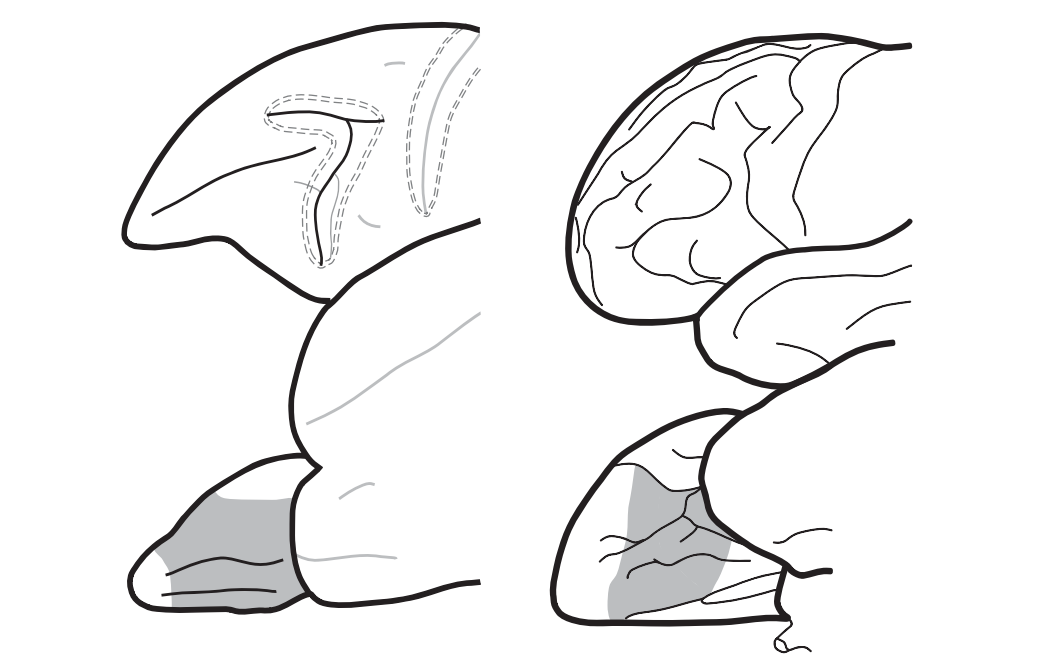
\includegraphics{image_pfc/Fig_4_1}
	\caption{猴子(左)和人类(右)的眶额皮层。 格式如图 1.2 所示。}\label{fig:fig_4_1}
\end{figure}



\section{连接}

图 \ref{fig:fig_4_2} 说明了眶额皮层的选定连接,这表明以下结论:\par


1. 与杏仁核最密集的连接涉及眶额皮层的颗粒部分,优先与杏仁核的基底外侧核连接。
然而,13 区的颗粒状部分也与杏仁核有关,其他粒度细分(见图 \ref{fig:fig_3_3})(Carmichael \& Price 1995a)。\par


\begin{figure}[!htb]
	\centering
	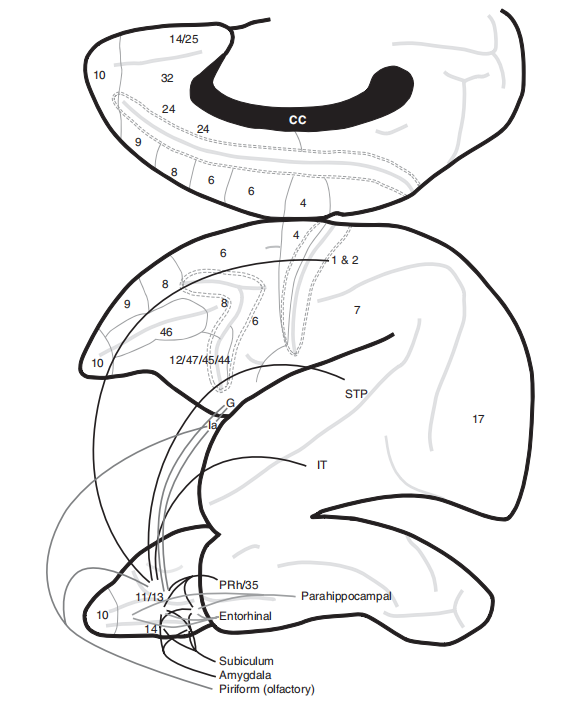
\includegraphics{image_pfc/Fig_4_2}
	\caption{眶额皮层的选定连接。 图 1.4 和 1.5 给出了脑沟和区域的名称。 线连接一些与轨道有直接轴突连接的区域,除非另有说明,否则假设是相连的。}\label{fig:fig_4_2}
\end{figure}


2. 无颗粒岛叶皮层接收来自味觉和梨状(嗅觉)皮层(Carmichael \& Price 1995a)。
它还接收来自脑干和丘脑的内脏信号 (Ray \& Price 1992)。
后者包括传达反映动物新陈代谢状态的信号的感觉,例如,缺氧或低血糖,以及来自肺、心脏、压力感受器和消化道 (Craig 2002)。
这些发现导致了这样一种观点,即颗粒状岛叶皮质在内感受中发挥作用。\par


3. 嗅觉、味觉和内脏信息从其到达颗粒状 OFC颗粒部分(Carmichael \& Price 1994)。
该信息可以在颗粒皮层中与来自颞下皮层的视觉输入相结合,目标区域 13 和 11,以及从投射到区域 13 的鼻周皮质(Saleem 等人,2008 年)。
后一种投影提供了关于物体的多模态信息 (Murray et al.
2007 年)。\par


4. S1区和S2区的体感信息也会传到13区,尤其是那些代表喙部(Pritchard et al. 1986)、唇和舌的侧面部分(Carmichael \& Price 1994)。
这些联系包括不明确的体感诸如顶叶盖和岛叶颗粒异常部分的区域皮层 (Saleem et al. 2008),以及定义明确的体感区域,例如区域3b 和 S2 本身。
与 S2 的某些联系可能涉及手和口面部表征 (Carmichael \& Price 1994)。\par


5. 与内侧前额叶皮层和腹侧前额叶皮层(第\ref{chap:chap3}章和第\ref{chap:chap7} 章)不同,眼眶PF皮质只有有限的听觉输入 (Saleem et al. 2008)。
14区的部分地区其中 13 个与可能提供听觉输入的颞叶区域有联系 (Petrides \& Pandya 1988)。
但是萨利姆等人。(2008) 重新诠释这些连接是根据他们识别的两个连接网络来表示的:轨道和中间网络。他们认为与听觉相关的区域要么是媒体网络的一部分,要么是两个网络的一部分。
根据这种观点,眼眶PF皮层的“纯眼眶”部分缺乏听觉输入。
原因大概是轨道网络处理有关物体(例如食物)的信息,这些物体具有很少有听觉特征。\par


这些点构成了眼眶 PF 皮层的连接指纹,这表明它是视觉信息与味觉信息汇聚的最早场所,嗅觉和内脏输入。
我们认为大多数视觉输入到达很重要。在灵长类动物特有的颗粒状区域。
因此它不是眶额前额叶皮层,一般来说,但特别是区域 13 和 11 的颗粒状部分似乎是视觉、嗅觉、味觉和内脏输入之间会聚的最听觉位置。\par


由于这种融合,特定食物的视线,例如特定成熟的阶段的水果,可以唤起它的味道和气味,这构成了它的味道,连同摄入后的内脏感觉。
此外,眼眶 PF 皮层接收来自初级体感皮层的口、唇和舌表征的输入(S1):与食物和液体摄入最相关的身体部位(Carmichael\& 价格 1995b)。\par


它的连接解剖结构使眶额前额叶皮层处于一个独特而有趣的位置。
触觉输入提供有关外部环境附近部分的信号;
视觉和嗅觉输入传递来自外部世界遥远部分的信号;
内脏输入告诉动物有关其内部环境的信息;
味觉和口腔体感输入告诉它有关从外部进入内部世界的事物。\par


图 \ref{fig:fig_4_3} 显示了这些不同的模态和子模态如何组合起来形成联合表征。
其中一些连接发生在无颗粒区域,它们似乎非常适合早期哺乳动物的谷物和昆虫饮食。
这些是专门从事夜间觅食以避免捕食等因素的小动物。
因此,在眶额前额叶皮层的颗粒部分中表示的连词主要涉及味觉、嗅觉和内脏感觉。
灵长类动物灵长类动物保留了这种基本的特征连接机制,并增加了更大的来自视觉区域的输入。\par


\begin{figure}[!htb]
	\centering
	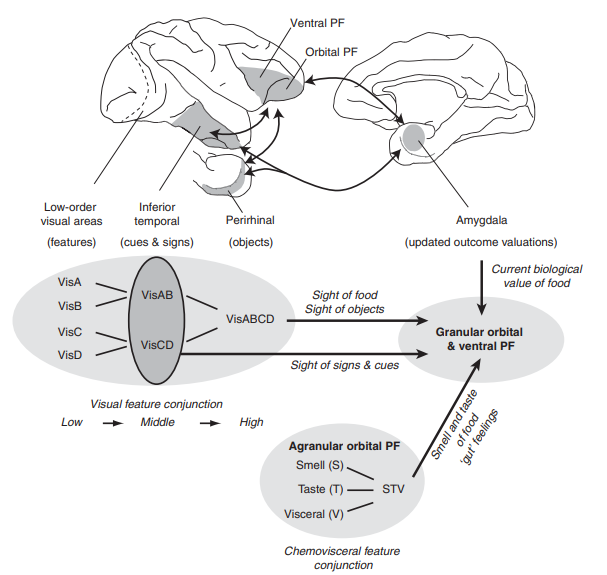
\includegraphics{image_pfc/Fig_4_3}
	\caption{颞叶和额叶皮层的特征连接。 VisA …VisD 指定视觉
		对象的特征,可以组合成各种连接表示,例如 VisAB,
		这表示 VisA 和 VisB 的表示。 “STV”表示物体的气味 (S)、味道 (T) 和内脏 (V) 特性的结合。 转载自 Murray EA, Wise SP,
		Rhodes SE,不同的大脑可以用奖励做什么? 在感觉神经生物学和
		奖励,编辑。 JA Gottfried © 2011,Taylor 和 Francis,经许可。}\label{fig:fig_4_3}
\end{figure}



\subsection{概括}

第 \ref{chap:chap3} 章认为——通过与海马体、杏仁核和内侧运动前区的联系——内侧前额叶皮层会偏向于在动作之间或在动作之间的选择有关行动的规则。
在那里,我们审查了证据表明它是基于预测结果的当前值这样做的,尤其是当这些选择取决于“内部”信号而不是感官信号时。
本章认为眶额前额叶皮层执行在外部信号之间进行选择的类似功能,尤其是那些来自物体的信号。
它之所以能够这样做,是因为来自体感、味觉、嗅觉、内脏和视觉皮层以及杏仁核的信息会聚和整合。



\section{啮齿动物的无颗粒皮质}

颗粒状前额叶皮层在啮齿动物研究中引起了相当大的关注,其中大部分表明在以结果为导向的行为中起着重要作用。
回想一下,在整本书中我们都区分了目标和结果,因此在其他人可能会说目标导向的地方使用术语“以结果为导向”。
眶额前额叶皮层细胞的活动反映了结果预测,尤其是关于奖励的特定感官方面的预测(Schoenbaum 等人,1998 年),这些区域的损伤会损害基于以下因素的选择
结果预期,如下一节所述。



\subsection{刺激-结果关联}

正如第 \ref{chap:chap3} 章提到的,当前的生物学需求会影响结果的评估。
例如,当前对食物或液体的需求越大,a 的值就越大映射到该结果的刺激。
将食物消耗到饱腹感会使该食物贬值,并且还有其他方法可以改变结果的价值。\par


在使用这些替代方法之一降低食物奖励价值的实验中,加拉格尔等 ( 1999 ) 比较了具有颗粒状前额叶皮层损伤的大鼠的行为与正常大鼠相比。
首先,他们教老鼠光表示食物供应。
当灯亮时,老鼠会靠近灯。
然后加拉格尔等人。
用过的锂氯化物诱发胃肠道疾病,这一过程称为条件性味觉厌恶。
稍后进行测试时,在所有疾病痕迹消失后,正常老鼠接近光线比他们生病前更少,或者完全停止接近光线。
受伤的老鼠表现不同。
他们比过去更频繁地接近光正常老鼠。
正如第 \ref{chap:chap3} 章所解释的,正常大鼠的结果称为贬值影响。
因为受损的老鼠接近了与奖励贬值相关的刺激,可以说,他们在使用刺激-结果关联来判断方面存在缺陷指导行动。\par


皮肯斯等人( 2003 , 2005 ) 使用相同的任务和贬值程序,但对杏仁核和颗粒状 OFC 造成损伤。
两个病变都废除了大鼠的贬值效应。
这些老鼠的行为就好像它们没有从它们身上学到任何东西一样疾病。\par


这些贬值程序的结果类似于第 \ref{chap:chap3} 章描述的结果对于内侧前额叶皮层的病变。
内侧前额叶皮层损伤会导致使用结果预测在竞争行为中进行选择时出现障碍。
在许多这样的实验中,没有任何外部提示可以帮助动物做出选择。
颗粒状眶额皮层病变,但是,不要破坏这种行动-结果关联(Ostlund \& Balleine 2007)。
相反,它们破坏了使用关于结果的预测来在对象中进行选择。
在这些实验中,外部提示会提示选择,从而揭示缺陷学习刺激-结果协会。
这些研究表明,颗粒状 OFC将刺激与结果联系起来,尤其是食物的感官方面,例如它的气味或味道。\par


伯克等人的一项实验( 2008 ) 支持这一结论。
老鼠首先学会了将一种刺激与一种特定的食物联系起来。 后来他们看到了这种刺激与额外刺激的结合。
当老鼠看到这种复合刺激时,它们得知它与另一种食物有关。
这两种食物有更多或不太一样的适口性和可取性,但它们的味道不同。\par


伯克等人发现大鼠将第二种食物的发生归因于复合刺激的较新部分。
作为这一结论的证据,他们表明他们的老鼠会按下一根杆来产生额外的刺激。
至关重要的是,Burke等人表明如果老鼠在第二次吃饱了就不太可能这样做食物。
因此,老鼠不仅将额外的刺激与第二种食物联系起来,而且使用该关联来评估刺激的当前值。
具有颗粒状 OFC 损伤的大鼠未能显示出这些效果。
关系在复合刺激的较新部分和特定感觉特性之间第二种食物不再影响他们的行为。
这些结果表明颗粒状眶额皮层介导刺激和结果之间的映射,尤其是结果的特定感官方面。\par


稍后,我们强调了粒度眶额皮层的重要性和视觉上的进步
灵长类动物。
然而,正如刚才回顾的实验所表明的那样,老鼠也使用视觉评估结果的刺激,他们的眶额皮层从视觉皮层区域接收到这些刺激。\par



\subsection{费用}

第 \ref{chap:chap3} 章解释了动物不仅根据预测的食物或液体做出决定,而且还有获得它们的成本。
例如,与正常大鼠相比,前扣带回晚期皮质受损的大鼠选择越过障碍的次数较少,因此似乎高估努力成本。\par


无颗粒眶额皮层的损伤也改变了大鼠估计成本的方式。
当在立即的小奖赏和延迟的大奖赏之间做出选择时,正常老鼠在做出选择时会考虑延迟的时间长短。
鲁德贝克等( 2006b ) 报道有眼眶 PF 损伤的大鼠更多地选择小的即时奖励经常比正常老鼠。
“冲动”一词已被应用于选择小额奖励很快,并且“耐心”一词已被用于放弃立即奖励以获得一个更大的以后。
所以在 Rudebeck 等人的实验中,眶额皮层眼眶病变可以据说会诱发冲动。\par


然而,只要稍微改变实验设计,就会得到不同的结果。
鲁德贝克等使用了 T 型迷宫,但 Winstanley 等人( 2004 ) 让老鼠在两个杠杆之间进行选择,一个导致单个颗粒,另一个在延迟后导致四个颗粒。 
眶额皮层病变的大鼠比正常大鼠更频繁地选择延迟奖励的杠杆。
有人可能会说他们表现出比正常人更多的“耐心”。
和马里亚诺等人 ( 2009 ) 让老鼠在 T 迷宫上的黑色或白色目标框之间做出选择,一个框内有小奖励,另一个框内有大量奖励,只有在延迟后才能获得。
同样,患有眶额皮层病变的大鼠比 Rudebeck 等人研究中的大鼠表现出更多的“耐心”。\par


泽布等人 (2010) 表明,眶额皮层病变是否会导致“冲动”或“患者”选择取决于两个因素:
一个明确的信号,表明个体大鼠之间的延迟和差异。
他们使眶额皮层失活并比较了提示的效果和无意识的延误。
他们的结果表明,对于明显有提示的延迟,失活会增加立即奖励的选择(冲动),而对于无提示的延迟,失活会减少立即奖励的选择(耐心),但仅限于有强烈冲动倾向的老鼠个体。
所以我们不能简单地说大鼠眶额皮层偏向于冲动或耐心觅食的选择。
但是,它显然以某种方式在评估延迟成本方面发挥了作用以及偏向延迟或立即行动的行为。
正如第 \ref{chap:chap3} 章所解释的那样,累加器-跑道模型提供了一种实现这种偏差的简单机制,既可以通过改变产生输出的阈值,也可以通过调制速率支持进行特定运动的“证据”不断积累. \par


冲动觅食和耐心觅食之间的竞争通常是根据延迟或远距离获得的食物和液体的贬值或折扣来讨论的。
然而,正如斯蒂芬斯等人( 2004 ) 指出,这个术语意味着动物错误地评估了时间和空间上遥远的食物和液体的价值。
或者,动物可能会准确评估价值,但会考虑寻找遥远可用资源的固有风险。 \par


Hayden 和 Platt (2007) 建立了一个模型,其中“风险”期权的估值取决于较大收益的预期时间和收益减少的风险。
他们表明,该模型的预测解释了猴子在赌博任务中做出的选择。
由于等待更长时间或走得更远所固有的风险,选择开发立即可用的资源并不一定意味着对延迟或更远资源的错误评估。
即使眼前的补丁比别处的“更绿的牧场”价值低,回报更确定。



\subsection{颗粒状岛叶皮质}

基于连接、细胞结构和拓扑结构,眼眶 PF 皮层包括无颗粒岛叶皮层 (Carmichael \& Price 1994)。
如果无颗粒眶额皮层将刺激与结果的特定感觉方面相关联,我们可能期望找到邻近的无颗粒岛叶皮层的相关功能。
Balleine 和 Dickinson (2000) 表明,具有包括无颗粒岛叶皮层在内的损伤的大鼠在需要记住特定味道时表现出损伤。
他们在两种情况下对老鼠进行了测试。
在其中一项中,老鼠在两个杠杆之间做出选择,并接受了那种与任一选择相关的食物。
受损的老鼠倾向于避免按下刚刚导致奖励贬值的杠杆。
在第二种情况下,压榨机不再生产任何食物;
也就是说,老鼠在灭绝中进行了测试。
在这种情况下,受伤的老鼠同样地按下了两个杠杆。\par


因为其他实验表明有这些损伤的老鼠可以学习这种消退任务,Balleine 和 Dickenson 得出结论,有损伤的老鼠无法回忆起它们期望通过按下每个杠杆获得的食物的特定感官特性,因此,尽管其中一种食品贬值,但他们同样选择了它们。
尽管他们的病变侵入了位于岛叶皮质皮质尾部的味觉皮质,但这种影响可能是由岛叶皮质皮质病变引起的。\par


Kesner 和 Gilbert (2007) 还测试了老鼠预期奖赏的能力。
老鼠先喝低蔗糖液体,然后喝高蔗糖液体,几天后,它们喝的低蔗糖液体减少了,以便以后消耗更多的高蔗糖液体。
无颗粒岛叶皮层的损伤消除了这种效应。
然而对照试验表明,受损的大鼠仍然可以分辨出两种液体之间的差异。
本实验表明,岛叶皮质受损的大鼠倾向于选择即时奖励,而不是等待更高价值但延迟的奖励。
这结果可能反映出未能预测延迟奖励的属性或冲动的选择。\par



\subsection{概括}

按照本章第 \ref{chap:chap3} 章所述,内侧前额叶 皮层的颗粒部分似乎使用行动-结果映射和动机评估来偏向行动或有关行动的规则之间的选择。
映射和估值都涉及“内部”信号,两者都可以影响代表特定选择的累加器网络中的活动(第 \ref{chap:chap3} 章)。
因此,例如,按下杠杆预测有益结果(例如葡萄干)的“内部”信号以及评估该结果的信号就当前需求而言,两者都为代表压杆行为的累加器网络提供了“证据”。
有了更多这样的“证据”——例如,更强的关联或获得葡萄干的更高动机——网络将更快地达到阈值并“赢得”控制行为的“竞赛”。
相比之下,眼眶 PF 皮层的颗粒部分似乎使用刺激-结果映射以及动机评估来偏向刺激之间的选择。
与行动-结果映射不同,刺激-结果映射依赖于外部的、感官的信号以及内部信号(关于动机),它们也可以影响累加器网络中的活动。
因为这些区域通过它们密集的互连一起工作(Barbas 1988 ;Price \& Drevets 2010),它们允许哺乳动物选择预测最佳结果的行动或刺激,根据当前的动机价值更新。
我们认为,这种能力比缺乏这些皮层区域的祖先物种更具优势(第 \ref{chap:chap2} 章)。
由于它们的无颗粒 PF 皮层,哺乳动物可以在面对不断变化的环境时迅速改变觅食选择。
上一章表明,他们可以学习习惯应该盛行或以结果为导向的行为应该盛行的环境,他们可以学习何时应该通过内在或外在规则来引导导航,并且他们可以通过努力来权衡奖励收益 费用。
本章表明他们可以了解“冲动”或“耐心”觅食的背景。
从这个意义上讲,哺乳动物可以获得相互矛盾的行为知识,当环境发生变化时,它们可以用来偏向其他行为控制系统。
第 \ref{chap:chap3} 章解释了这如何在神经网络层面发挥作用。
表 \ref{tab:tab_4_1} 总结了这些与觅食选择相关的想法。
它并不意味着详尽无遗。
例如,我们忽略了巴甫洛夫到工具的转移、差异结果效应和条件强化等现象。
啮齿动物的颗粒状 OFC 损伤会导致这些任务以及本章和表 \ref{tab:tab_4_1} 强调的任务受损。



\begin{table}[htbp]
	\newcommand{\tabincell}[2]{\begin{tabular}{@{}#1@{}}#2\end{tabular}} %换行指令
	\centering
	\caption{颗粒状 PF 区域对觅食选择的贡献}
	\renewcommand\arraystretch{1.5}	%设置表格内行间距
	\begin{tabular}{llll}
		\toprule 
		区域   &  贡献  \\
		\midrule
		\tabincell{c}{内侧颗粒状PF\\}&根据预测的成本/收益,在多种行动选择中偏向觅食\\&在中等波动环境中偏向于以结果为导向的选择\\&偏向低波动环境的习惯觅食\\&偏向于外在或内在的导航规则\\
		\midrule
		\tabincell{c}{眶额颗粒状PF}&基于结果的预测感官方面的多种刺激之间的偏差觅食\\&偏向于“冲动”觅食以利用可用资源\\&偏向“耐心”觅食以探索遥远的资源 \\ 
		\bottomrule
	\end{tabular}%
\label{tab:tab_4_1}
\end{table}%



\section{灵长类动物的颗粒区域}

第 \ref{chap:chap2} 章和第 \ref{chap:chap3} 章讨论了啮齿动物的内侧额叶皮层与灵长类动物的中外侧前额叶皮层(46 区)同源或类似的说法。
没有令人信服的证据支持这一建议,很多人反对。 在这里我们简要地处理一个关于眶额皮层的相关争论。\par



\subsection{比较啮齿动物和灵长类动物的颗粒区域}

与灵长类动物的眶额皮层不同,大鼠的眶额皮层完全没有颗粒。
此外,它具有非常类似于颗粒状但不是颗粒状的连接,部分灵长类眶额皮层。
与粒状前额叶皮层不同,它位于 allocortex 附近,并且与粒状前额叶皮层不同,它对自主输出有相对直接的影响。\par


然而,尽管有所有这些证据,一些神经科学家认为大鼠的颗粒状眶额皮层对应于猴子的整个眶额皮层,包括其颗粒区域(Uylings 等人 2003 年;Seamans 等人 2008 年;Schoenbaum 等人2009).第 \ref{chap:chap2} 章解释了这个想法采用两种形式之一。
一是老鼠有猴子眶额皮层的微型复制品;
另一个是他们融合了所有领域发生在猴子身上。
这两种观点都基于大鼠和猴子眶额皮层之间的某些相似性,例如细胞活动、神经化学特性、连接和损伤效应。
但是所引用的相似性并不对应于诊断特征,而诊断特征正是建立同源性所需要的。
正如第 \ref{chap:chap2} 章和第 \ref{chap:chap3} 章所讨论的,诊断特征将不同的区域区分开来。
以条件反射的消失为例。
尽管有眶额皮层 损伤的大鼠表现出比正常消退慢(Kolb 等人 1974年),但猴子中仅限于颗粒状眶额皮层的损伤具有相同的效果(Izquierdo 和 Murray 2005 年)(图 \ref{fig:fig_4_4}),包括颗粒状眶额皮层 的损伤也是如此 猴子(Butter 1969)。
因此,有问题的相似性——称为眶额皮层的区域的病变导致灭绝学习减慢——无助于我们建立同源性。\par


\begin{figure}[!htb]
	\centering
	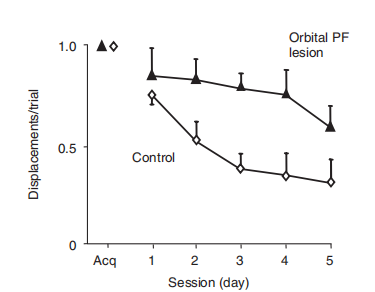
\includegraphics{image_pfc/Fig_4_4}
	\caption{猴子眶额皮层颗粒损伤导致的消退学习减慢。 猴子优先
		学习移动物体以获得食物奖励。 在这个收购 (acq) 阶段,
		猴子在每次试验中有 30 秒的时间来移动物体,而且它们在每次试验中都会这样做。 在随后的测试阶段,称为消光试验,取代该物体永远不会产生食物。 正常(对照)猴子将他们的位移减少到试验的一半以下5天的测试。 具有颗粒状眶额皮层损伤的猴子以高于正常的猴子,尽管经过 5 天的测试后它们有了显着改善。 修改自Izquierdo A, Murray EA。 杏仁核和眼眶前额叶皮层损伤的相反作用
		猕猴乐器反应的灭绝。 欧洲杂志神经科学 22:2341–6,© 2005,John Wiley and Sons,经许可。}\label{fig:fig_4_4}
\end{figure}



\subsection{细胞活性}

不幸的是,除了我们之前回顾的解剖学知识外,我们对灵长类动物眶额皮层的颗粒部分知之甚少。\par


罗尔斯等人 ( 1994 ) 记录了眶额皮层中对咸味、苦味、酸味和涩味做出反应的细胞。
从我们对它们记录位置的检查来看,它们似乎主要记录了 13 区和 14 区的颗粒部分,在 13 区的颗粒部分和岛叶皮质的颗粒部分也有额外的细胞群。所有这些区域的细胞都会对口味做出反应。\par


除了味觉输入,视觉和嗅觉输入有助于确定食物和液体的特性。
在 Rolls 和 Baylis 的研究中,眶额皮层中的细胞对视觉和味觉的结合以及嗅觉和味觉的结合都有反应。
大多数显示味觉-视觉或嗅觉-视觉连接的细胞发生在眶额皮层的尾端。
一些位于岛叶皮质的颗粒状区域,而另一些位于 13 区的颗粒状部分或至少附近。相同的特性发生得更多也位于眶额皮层。\par


Rolls 和他的同事还发现,猴子会按下一个杠杆,通过电极刺激第 13 区的颗粒状部分,这表明它们发现这种刺激是有益的(Mora 等人,1980 年)。
刺激 11 区没有这种效果。
所以细胞位于眶额皮层更靠后的部分,包括那些对味觉或视觉或气味与味觉的结合有反应的部分,似乎与大脑其他部位的奖赏系统的相互作用比眶额皮层的更靠侧部分更直接。\par



\subsection{概括}

啮齿类动物和灵长类动物都有一个无颗粒的眶额皮层(见图 \ref{fig:fig_2_1}),我们假设它的某些功能是从它们的共同祖先那里继承而来的。
不幸的是,我们几乎没有关于猴子眼眶无颗粒区域的直接损伤或细胞记录证据,因此我们承认这只不过是一种假设。
然而,我们确实知道颗粒区域具有密集的互连与颗粒区域,并且颗粒区域中的细胞具有我们在此基础上期望的感觉反应,例如用于识别特定食物和液体的视觉,气味和味道的结合。
当然,在实验室中,这些食物和液体可作为指导行为的结果。\par



\section{颗粒状皮质}

与灵长类动物中颗粒状 OFC 的信息匮乏相比,其颗粒部分已得到广泛研究。
我们根据损伤对刺激和结果之间的关联映射的影响、神经编码这些映射根据特定结果和“通用货币”、基于结果的规则选择、对这些结果的动机估值的更新以及将结果准确分配给选择。



\subsection{刺激-结果映射}

与其他动物一样,猴子使用刺激来预测结果并在此基础上做出觅食选择。
两种实验证明了这些预测:概率结果实验(图 \ref{fig:fig_4_5}B)和确定性结果实验(图 \ref{fig:fig_4_5}A)。
在前者中,猴子选择两种或多种产生奖励概率不同的刺激中的一种;
在后者中,猴子学会在两种刺激之间做出选择,以始终获得奖励,并在奖励偶然性切换到替代选择时改变选择。\par


\begin{figure}[!htb]
	\centering
	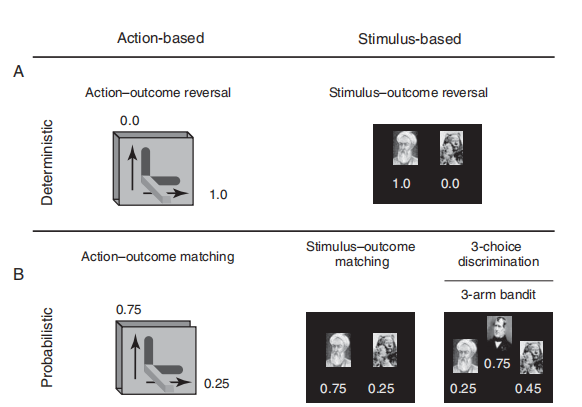
\includegraphics{image_pfc/Fig_4_5}
	\caption{区分基于动作(左)和基于刺激(右)选择的实验。 (一) 在
		基于确定性动作的选择(左),将手柄向右移动被描述为导致
		每次奖励,比例为1.0,而向上移动手柄永远不会产生奖励(0.0)。 这些结果后来在确定性动作逆转任务中切换。对于基于刺激的选择(右),猴子必须接触触摸屏上显示的两张图片之一。 每个选择的奖励概率是确定性的(0.0 或 1.0)。 (B) 在概率任务中,对于两个动作之间的选择,奖励的可能性在 0 和 1之间变化(左)或两个物体(中间)。 这些数字给出了每个选择获得奖励的试验比例。这些任务根据“匹配法则”称为匹配任务,而不是匹配样本任务。 在三选择辨别任务(右)中,也称为三臂强盗任务,三种选择中的每一种都以不同的概率得到回报,这种概率随时间而变化。 修改自	Rudebeck PH、Behrens TE、Kennerley SW、Baxter MG、Buckley MJ、Walton ME、Rushworth MF。额叶皮层子区域在行动和刺激之间的选择中扮演着不同的角色。 杂志神经科学 28:13775–85, © Society for Neuroscience, 2008, 经许可。}
	\label{fig:fig_4_5}
\end{figure}


鲁德贝克等( 2008 ) 使用概率方法。
在任务的一个版本中,称为刺激-结果匹配(图\ref{fig:fig_4_5}B),他们分配了四个概率级别,两个独立的概率算法确定两个刺激中每个刺激的级别。
一次该算法为刺激分配了一个概率,该概率在试验中保持不变,直到猴子选择了该刺激。
然后概率发生了变化,因此动物不得不根据它们的概率在刺激选择之间反复切换付清。
在另一个概率任务中,称为三臂强盗任务或三选择辨别任务,猴子学会在三种刺激中进行选择,每种刺激的奖励概率随试验次数而变化(图\ref{fig:fig_4_5}B)。\par


鲁德贝克等在受过训练以执行三臂强盗任务的猴子的颗粒状眶额皮层中造成损伤。
这些猴子调整他们的选择以改变奖励概率比正常猴子慢得多,这表明存在缺陷学习刺激和结果之间的关联映射(图\ref{fig:fig_4_6})。
或者,我们可以根据学习(或更新)选择和结果之间的关联映射来描述损伤。
在本章的其余部分,我们交替使用刺激-结果、对象-结果和选择-结果。\par


然而,当这些猴子通过选择两种行为中的一种而不是通过选择两种刺激中的一种来获得奖励时,它们表现正常。
该任务要求猴子选择抬起或转动杠杆以获得奖励,这是确定性动作逆转任务的概率版本第 \ref{chap:chap3} 章介绍。\par


除了患有颗粒状眶额皮层损伤的猴子,Rudebeck 等人在刺激-结果匹配任务中测试了前扣带回皮层损伤的 mon 键。
他们发现在这些内侧 PF 皮层损伤后刺激之间的转换没有受损,尽管 Kennerley 等人(2006) 表明,相同的病变会损害动作之间的切换。\par



鲁德贝克等得出的结论是,内侧前额叶皮层支持动作和结果之间的关联映射,而眶额皮层介导刺激和结果之间的关联映射。
但是 Rudebeck 等人和肯纳利等人报告了局限于前扣带回沟的皮质病变的 ed 结果。
对于较大的病变,尤其是那些同时包括前扣带回和前扣带回的病变,会出现更加复杂的情况。
E. A. Murray 等人(个人通讯)据报道,在这些较大的病变后,猴子在标准物体逆转任务中有损伤。
然而,Meunier 等人( 1997 ) 直接比较了有扣带回和眼眶 PF 病变的猴子的表现,有眼眶 PF 病变的猴子在物体反转任务上犯了两倍的错误。  \par


因此,物体反转任务继续对理解眶额皮层产生重大影响。
图 \ref{fig:fig_4_5}A 说明了这个确定性任务。
当发生反转时,奖励偶然性在两种刺激之间切换,通常除了奖励或非奖励反馈外没有任何其他提示。\par


在一项早期且有影响力的研究中,Butter (1969) 对猴子进行了三项任务测试:对象反转学习、空间反转学习和消退。
在一些猴子身上,他去除了眶额皮层,连同位于眼眶表面的 12/47 区部分半球的。
这些猴子在对象反转学习和消退学习上有障碍,但在空间反转学习上没有。
在其他猴子身上,他移除了腹侧前额叶皮层,包括整个 12/47 区。
这些猴子在灭绝任务。\par


许多随后的实验已经证实了眶额皮层和腹侧前额叶皮层之间的功能区别,以及在眶额皮层损伤后对象反转和消退学习的缺陷(Dias 等人 1997 年;Izquierdo 等人 2004 年)。
例如,腹侧前额叶皮层的损伤会在对象反向学习的初始阶段损害表现,但前额叶皮层损伤会导致更严重和更持久的损伤(Rygula 等人,2010 年)。\par


Butter 得出结论,眶额皮层的损伤会导致持续的行为障碍。
而且,从那时起,许多关于眶额皮层的研究都被解释为坚持、反应抑制和行为抑制 (Roberts \& Wallis 2000)。
根据这个想法,有缺陷的猴子在抑制先前获得奖励的选择方面存在缺陷,这会产生毅力。\par


Rudebeck 和 Murray ( 2008 ) 重新审视了这个话题,他们从几个方面进行了分析。
首先,在图\ref{fig:fig_4_7}所示的数据分析中,来自 Izquierdo 等人( 2004 ),他们计算了错误的总数,直到猴子完成了从选择先前奖励刺激到选择当前奖励刺激的转换。
正如预期的那样,Rudebeck 和 Murray 发现,双侧病变的猴子与正常猴子相比,眼眶 PF 皮层在两个物体之间的选择更慢。
此外,与正常猴子不同,如果对一系列逆转进行测试,则受损猴子无法通过这一系列对象逆转测试进行改进(图\ref{fig:fig_4_7})。\par


接下来,Rudebeck 和 Murray 逐个试验地分析了他们的结果,而不是像神经心理学家传统上所做的那样对试验块进行平均。
肯纳利等人( 2006 年 ) 他们对内侧 PF 皮层的动作逆转实验使用了相同类型的分析(第 \ref{chap:chap3} 章)。
Rudebeck 和 Murray 以两种方式测量了错误的数量,这两种方式都发生在刺激-结果映射发生逆转之后。\par


首先,如图 \ref{fig:fig_4_8}A 所示,Rudebeck 和 Murray 计算了第一个正确选择之前的错误数量,并将这些数据与第一个正确选择之后的错误数量进行了比较。
正常猴子和受损猴子之间的最大差异发生在第一次正确选择之后。\par


其次,如图 \ref{fig:fig_4_8}B 所示,作者研究了动物坚持正确反应的可能性有多大,作为最近奖励的函数,这是一种积极的反馈。
为此,Rudebeck 和 Murray 比较了一次试验后的性能错误,在错误纠正序列之后进行一次试验,在错误纠正序列之后进行一次试验,等等。
图 \ref{fig:fig_4_8} B 显示眼眶 PF 皮层的损伤导致使用正反馈的效率低下。
即使两个、三个或四个正确(并获得奖励)在错误之后做出反应,患有眼眶 PF 皮层损伤的猴子比正常猴子犯了更多的错误。
然而,他们的表现几乎正常,以回应来自无回报选择的负面反馈(Rudebeck \&Murray2008年)克拉克等人。
( 2008 ) 在狨猴中发现了类似的结果。\par


结合 Kennerley 等人的类似分析。 ( 2006)对于行动-结果学习,Rudebeck 和 Murray 的结果为解离提供了进一步的支持内侧前额叶皮层和眶额皮层之间的功能。
在图 \ref{fig:fig_4_5} 所示的任务系列中,眶额皮层的损伤导致学习改变的刺激-结果关联的障碍,但不影响改变的动作-结果协会。
相比之下,内侧前额叶皮层的损伤——更具体地说是前扣带回皮层的损伤——会导致学习改变的动作-输出映射的损伤,对学习刺激-结果的影响较小且不太可靠映射。\par


最近一项针对人类的病变研究得出了类似的结论。
卡米尔等人(2011) 研究了背侧前扣带皮层或前额叶皮层病变的患者。
对于后者,在颗粒状眶额皮层中发现了最大的重叠区域,靠近它与颗粒状眶额皮层的边界。
但在大多数患者中,病变涉及两个区域。
卡米尔等人。 使用与猴子实验相同的分析并发现相似的结果。
在刺激-结果任务中,受试者在一副彩色扑克牌中做出选择,这些扑克牌要么产生收益,要么损失 50 美元的游戏币。
一种颜色的一副牌在 86\% 的试验中获得收益,而另一种颜色在 14\% 的试验中获得收益。
在行动-结果任务中,受试者在前臂的旋前和旋后运动之间进行选择,结果相同。
科目后学会了正确的选择,意外事件就发生了逆转,就像在猴子实验中进行的行动逆转和对象逆转一样。\par


卡米尔等人测量了受试者在积极反馈后错误地改变了他们的选择的试验比例。
这种转变是错误的,因为反馈表明他们应该坚持之前的选择。
眶额皮层病变导致刺激-结果逆转受损,但这些患者在动作-结果任务中表现得像对照受试者(图 \ref{fig:fig_4_9})。
相比之下,与对照组相比,前扣带皮层损伤导致了行动-结果逆转的损害。
患有这些病变的患者在刺激-结果任务中也比对照组犯了更多的错误,但这种差异没有达到统计学意义(图 \ref{fig:fig_4_9})。\par


\begin{figure}[!htb]
	\centering
	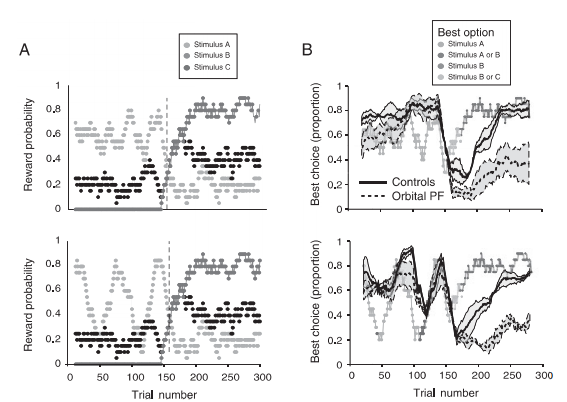
\includegraphics{image_pfc/Fig_4_6}
	\caption{猴子 OFC 颗粒状损伤后选择结果学习受损。 (A) 对于图中说明的任务,选择三个类对象刺激中的每一个的回报概率图 4.5 右下角,三臂老虎机任务。 回报率随试验的变化而变化数量,但不取决于猴子的选择。 (B) 猴子的试验比例根据收益概率评估做出最佳选择。 纵坐标表示正常(对照)猴子(实线)选择最高价值对象(最佳选择)的比例和有颗粒状 OFC 损伤的猴子(虚线)。 阴影:SEM。 任何试验中最佳刺激的回报概率以灰色绘制。 顶行:低波动性条件。 底部行:高波动情况。 转载自 Walton ME、Behrens TEJ、Buckley MJ、RudebeckPH、拉什沃思 MFS。 猕猴大脑中的可分离学习系统和眶额的作用皮质在偶然学习中。 神经元 65:927–39,© 2010,经 Elsevier 许可。}
	\label{fig:fig_4_6}
\end{figure}


\begin{figure}[!htb]
	\centering
	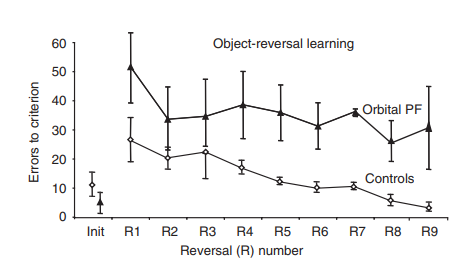
\includegraphics{image_pfc/Fig_4_7}
	\caption{颗粒状眶额皮层损伤后猴子的物体逆转功能受损。 数字错误标准性能的两个选择,确定性对象辨别任务。在初始训练(Init),没有逆转,猴子学会区分两个物体错误相对较少。 眼眶 PF 皮层在这种学习中不起作用,因为猴子只需要学习哪些对象是正值的,哪些是中性的。 一旦简单将物体分类为阳性或中性不再解决问题,因此眼眶 PF皮质变得必要。 R1. . R9 表示九个连续反转,其中随着时间的推移两个对象在交替的试验块中变得积极和中立。 有颗粒状病变的猴子眶额皮层学习这些逆转的速度比正常(对照)猴子慢,而且它们无法改善连续九次逆转。误差线:SEM。 转载自 Izquierdo A, Suda RK,默里EA。 恒河猴的双侧眼眶前额叶皮层损伤会扰乱由以下因素引导的选择奖励价值和奖励偶然性。 神经科学杂志 24:7540–8, © Society for神经科学,2004 年,经许可。}
	\label{fig:fig_4_7}
\end{figure}


\begin{figure}[!htb]
	\centering
	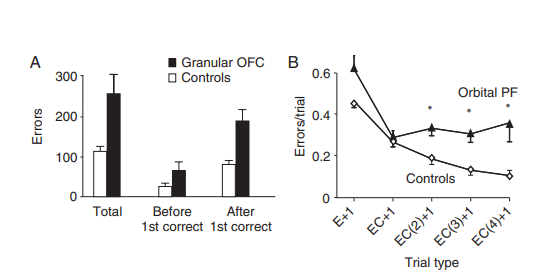
\includegraphics{image_pfc/Fig_4_8}
	\caption{(A) 在第一次正确选择之前和之后,在对象反转任务上犯的错误。 为了有颗粒状眶额皮层损伤的猴子(黑条)和正常(对照)猴子(白色条酒吧)。 大多数错误出现在第一个正确选择之后。 (B) 错误后的逐个试验性能(E + 1),在一系列错误之后是一个正确的选择 (EC + 1),在一个错误之后是两个连续的正确选择 [EC(2) + 1],等等。 粒状眶额皮层(实心三角形)无法像正常(对照)猴子(白色菱形)那样有效地受益来自奖励的积极反馈。 星号:统计显着差异。误差线:SEM。 转载自 Rudebeck PH、Murray EA。 杏仁核和眶额皮质在对象反转学习过程中,病变会不同地影响选择。 神经科学杂志28:8338–43, © Society for Neuroscience, 2008,经许可。}
	\label{fig:fig_4_8}
\end{figure}


\begin{figure}[!htb]
	\centering
	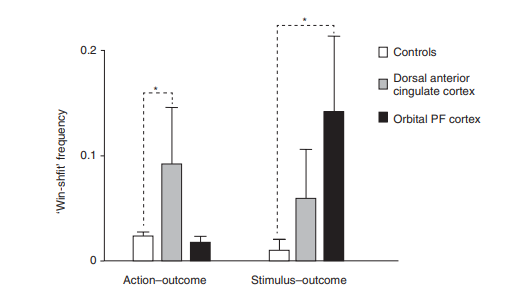
\includegraphics{image_pfc/Fig_4_9}
	\caption{眼眶 PF 皮层(黑条)和病变患者的逆转损伤与对照组(白色条)相比,前扣带皮层(灰色条)。 为了对象反转任务,受试者在不同颜色的牌组之间进行选择; 为了行动逆转任务,他们在旋前或旋后运动之间进行选择。在“胜利”之后换档,“win-shift”频率,与图 4.8 中猴子所说明的错误类型相同。 错误酒吧:SEM。 星号:统计上显着的对比。 转载自 Camille N, Tsuchida A,研究员LK。 人类刺激价值和行动价值学习的双重分离眶额或前扣带皮层损伤。 神经科学杂志 31:15048–52, ©神经科学学会,2011 年,经许可。}
	\label{fig:fig_4_9}
\end{figure}


除了证明眶额皮层和内侧前额叶皮层之间的功能分离外,Rudebeck 和 Murray 在猴子身上的发现以及 Camille 等人的发现。
在人类中证明,患有眶额皮层皮层损伤的受试者使用正反馈的效率低下,但几乎可以正常使用负反馈。
这些发现直接与眶额皮层损伤的受试者由于无法抑制习得反应而坚持不懈的观点相矛盾。
事实上,这些实验中的受试者改变了他们之前的选择几乎正常,基于负面(错误)反馈。
与坚持不懈不同,这种损害可以被描述为坚持不力:与坚持不懈相反。
第 \ref{chap:chap10} 章更详细地讨论了行为抑制和坚持以及整个前额叶皮层。
在对象反转实验中,猴子会收到两种反馈,表明刺激-结果映射已发生变化:预期奖励未发生或意外奖励发生。\par
这两种情况都会导致“奖励预测错误”(Schultz \& Dickinson 2000)。
对中脑多巴胺能神经元的研究表明,当意外奖励到来时,活动会增加,而当预期奖励未能实现时,活动会减少 (Schultz 1998)。
在第 \ref{chap:chap3} 章中,我们将此属性称为有符号误差信号,以便将其与内侧前额叶皮层中出现的无符号误差信号进行对比。
多巴胺能细胞将它们的轴突发送到纹状体和皮质,以及其他大脑结构,这些结构使用这些带符号的错误信号来调整行为。\par


奥多尔蒂等人( 2003 ) 使用了一种时间差分学习模型,该模型取决于奖励预测误差。
他们在执行一项使用复杂的颜色和形状模式作为刺激的任务时扫描人类受试者。
其中一个刺激信号发出一滴甜味液体的信号,第二个刺激信号表示没有液体,第三个刺激信号发出中性味道的液体信号。
然而,在一些试验中,预测的事件没有发生。
奥多尔蒂等人。 寻找与签名奖励预测错误信号预期模式相匹配的激活:
当甜味未能按预期发生时激活减少,而当甜味意外发生时激活增加。
眶额皮层和纹状体腹侧部分的激活与这种模式相匹配。
当然,这些信号也可以在前额叶皮层的其他部分找到。 如第 \ref{chap:chap3} 章提到,猴子内侧前额叶皮层中的神经元也编码各种奖励预测错误(Matsumoto 等人 2007 年;Seo 和 Lee 2007 年;Hayden 等人 2011a)。
然而,对于内侧前额叶皮层,错误信号似乎主要涉及动作之间的选择,而在 O'Doherty 等人的影像学研究中 ( 2003 ) 他们涉及刺激之间的选择。\par



\subsection{编码刺激-结果映射}

第 \ref{chap:chap3} 章解释了内侧前额叶皮层中的细胞具有反映视觉刺激价值的活动,包括成本和收益。
正如我们在那里提到的,类似的活动发生在眶额皮层中。 
肯纳利等人( 2009 ) 例如,研究了奖励金额、奖励概率和多次按键的努力成本等变量。
当猴子必须在不同价值的刺激之间做出选择时 (Seo \& Lee 2008) 以及当它们只是观察刺激和价值之间的关联时,眶额皮层中的细胞编码这些变量,就像在巴甫洛夫条件反射中发生的那样 (Morrison \& Salzman 2009)。\par


简而言之,文献表明,眶额皮层的神经元活动不仅编码物体和奖励的价值 (Padoa-Schioppa \& Assad 2006) 和获得奖励的概率 (Kennerley et al. 2009),而且还编码 影响觅食选择的许多其他因素。
这些因素包括有益和有害的结果 (Morrison \& Salzman 2009),包括努力成本 (Kennerley et al. 2009)、时间 (Roesch \& Olson 2005) 和风险 (O'Neill \& Schultz 2010),以及 结果会出现拒绝选择 (Abe \& Lee 2011) 和对选择成功的信心 (Kepecs et al. 2008)。\par


相关的神经生理学研究强调了相对价值,这反映在对不同种类食物和液体的偏好上。
Tremblay 和 Schultz (1999) 研究了颗粒状眶额皮层中的神经元活动。
例如,当猴子在苹果和谷物之间做出选择时,细胞可能对苹果有更大的反应,但当猴子在香蕉和苹果之间做出选择时,细胞对苹果的反应可能更小。
这些细胞编码食物的相对价值。
除了相对估值外,颗粒状眶额皮层中的一些神经元编码独立于可用选择的值(Padoa-Schioppa 2009)。
这些属性来自连接,但内侧前额叶皮层中的细胞也编码刺激预测结果的值似乎令人费解(Kennerley 等人,2009 年)。
激活也发生在内侧前额叶皮层以选择对象(Behrens 等人 2007 年;Glascher 等人 2009 年),并且那里的损伤可能会对对象选择产生一些影响(Camille 等人 2011 年)。
乍一看,行动-结果和刺激-结果编码之间的严格二分法似乎排除了这些结果。
如前所述,眶额皮层的损伤导致物体之间逆转的损伤(Rudebeck 等人 2006b),而内侧前额叶皮层的损伤导致动作之间逆转的损伤(Kennerley 等人 2006)。\par


基于这些结果,人们可能会假设内侧前额叶皮层应该缺乏反映刺激-结果结合的活动。
然而,第 \ref{chap:chap1} 章解释了为什么病变研究会产生与记录或成像结果似乎不一致的结果,至少在表面上。
部分原因在于眶额皮层和内侧前额叶皮层协同工作。
通过密集的互连,他们可以将刺激-结果连词与行动-结果连词结合起来。
可供性的概念有助于解释这些高阶表示。
术语可供性指的是与一个对象或一类对象相关联的动作。通过结合对象-结果和动作-结果关联,内侧前额叶皮层可能编码与以某种方式作用于对象相关的结果,在对象操作期间发生。
因此,这些表示包括对象的特征和与对象相关联的动作。
这个想法可以解释为什么对象值连接在内侧前额叶皮层中如此突出;
对象可以参与许多不同类型的动作。
这些细胞也可能编码比具体的行动-结果关联更抽象的东西,例如预测对某个对象进行任何操作或对它进行某类操作的结果。\par


如果内侧前额叶皮层的某些部分代表动作、物体和结果的结合,这可能解释了成像和细胞记录结果,以及内侧前额叶皮层损伤对物体选择的不一致影响。
例如,我们前面提到了一些未发表的证据,表明大的前扣带回损伤会损害物体反转学习(E. A. Murray,个人通信),尽管在类似的任务中猴子在较小的损伤后正常执行(Rudebeck 等人 2006b)。\par


内侧前额叶皮层和眶额皮层功能之间的严格二分法似乎也与另一个结果不一致。
正如内侧前额叶皮层中的细胞反映刺激-结果关联(Kennerley 等人 2009),眶额皮层皮层中的细胞反映动作-结果关联。
Tsujimoto 等人( 2009 ) 表明,颗粒状眶额皮层中的细胞编码猴子的动作选择,但仅在反馈(奖励或无奖励)发生的时间左右。
这些发现与病变的发现并不矛盾。
Tsujimoto 等人实验中的猴子。
在每次试验期间在视频监视器上保持可见的两个可见对象(白色方块)之间进行选择。
因此,有人可能会争辩说,细胞在反馈时编码了对象之间的选择,我们稍后会再次讨论这一发现。\par


我们的核心原则之一是,眶额皮层皮层的连接解释了为什么只有它才能执行其功能。
眶额皮层而非内侧前额叶皮层接收来自颞下皮层的输入,后者代表物体的颜色、形状和视觉纹理。
眶额皮层而非内侧前额叶皮层接收来自皮层味觉、内脏和嗅觉区域的直接输入,所有这些都与特定结果相关。
因此很容易理解为什么眶额皮层代表刺激-结果的结合,以及为什么它在根据结果选择对象方面起着必要的作用。\par



\subsection{以共同货币计价}

动物必须能够比较不同资源的价值,因为觅食选择通常涉及权衡取舍。
例如,动物可能既渴又饿。
有多少特定的液体在动机上等同于一定量的食物? 一
可能是动物以“通用货币”代表一切事物的价值,以便做出这样的选择。
这个想法是,选择的不同潜在结果,例如性、温暖和食物,在一个维度中表示,以指导选择(Montague \& Berns 2002)。
奖励预测误差信号具有此属性。
如果神经表征中存在“通用货币”,那么无论奖励的性质如何,我们都应该看到对不同类型的同样偏好的奖励做出类似程度的反应。
Padoa-Schioppa 和 Assad (2006) 在编码果汁价值的猴子眶额皮层,与果汁的种类无关。
从这个意义上说,一些眶额皮层细胞编码奖励的抽象价值:以通用货币奖励。\par


对于人类主体来说,金钱作为一种奖励,它的抽象性在于它可以换取多种商品。
奥多尔蒂等人( 2001 ) 教人类受试者一项针对金钱奖励的视觉辨别任务,收益与损失的激活在于头侧腹内侧 前额叶皮层,14 区。Kim 等人。 ( 2011 ) 在受试者看到视觉刺激时对其进行扫描,其中一些与不同数量的金钱相关,另一些与不同数量的果汁相关。
里面有激活腹内侧前额叶皮层(14 区)与钱的数量和果汁的数量有关。\par


同样,Sescousse 等人( 2010)将金钱的激活与色情刺激的激活进行了比较,认为后者对应于主要奖励。
他们发现了一个 rostro 尾部组织,其主要奖励导致尾部和更抽象的激活,“共同货币”奖励导致吻侧激活。
其他人也提出了类似的建议 (Kringelbach \& Rolls 2004)。\par


显然,以通用货币计算估值的能力具有优势。动物经常需要平衡各种成本和收益。
并且,在某个水平,一个完全处理单一维度的觅食结果的系统可以有效地发挥作用。
用关于特定结果的高维信息增强这个系统也提供了优势,特别是对于了解对比结果之间。
稍后我们讨论证据表明眶额皮层的外侧部分以高维方式编码输出,而内侧部分以单一方式编码结果“共同货币”维度。\par


除了正面估值外,颗粒状的眶额皮层也在负面估值中发挥作用。
例如,在对蛇恐惧的研究中,猕猴伸手越过中性物体或橡皮蛇取回食物。
正常的猴子只能越过蛇经过长时间的拖延,有时甚至根本拒绝这样做。
颗粒状眶额皮层损伤后,然而,猴子很快就伸手去拿食物,拿中性物体也一样和蛇 (Izquierdo et al. 2005)。
对这一结果的一种解释是,猴子没有对蛇的负估值进行编码。
\par



\subsection{基于结果的视觉规则}

在目前给出的示例中,相关结果涉及对象的表示,无论是食物、果汁还是金钱。
但人们也可以将结果与更抽象的事物联系起来表示,例如规则的表示。
用于辨别这些映射的测试是类似的,也。
正如实验可以评估猴子之间切换的能力一样对象之间的选择,因此可以评估在规则之间切换的能力。\par


巴克利等人( 2009 ) 研究了学习了样本匹配任务的猴子涉及两种不同的匹配规则。
样本刺激出现后经过一段延迟后,猴子面临三种选择刺激。
潜在选择之一匹配样品的形状,另一个匹配它的颜色,第三个匹配既不是形状也不是颜色。
猴子必须使用两个匹配规则之一:匹配形状或颜色匹配。
首先,他们学习了一条规则以达到高水平的表现,然后实验者改变了这条规则。
在随后的一系列试验中猴子不得不使用新建立的规则,除了奖励或非奖励之外没有其他提示来指导它们。
这些实验类似于对象反转和动作反转前面描述的任务。\par


为了研究眶额皮层损伤的影响,Buckley 等人。
采用了与 Rudebeck 和 Murray (2008) 使用的相同的逐个试验分析,本章前面部分对此进行了解释。
该分析衡量动物坚持正确规则的可能性有多大作为最近奖励的函数。
规则更改后,Buckley 等人。
比较性能错误后进行一次试验,错误纠正序列后进行一次试验,依此类推。
前在病变处,猴子在错误纠正序列后的正确率为 77\%。
那也就是说,他们使用正确试验的积极反馈来提高他们的表现,下次他们必须在两种视觉规则之间做出选择。
眶额皮层损伤后,在错误纠正序列之后,猴子的表现只有 50\% 是正确的。
这一发现表明眶额皮层在将结果与选择相关联方面起着重要作用,规则之间以及对象之间的选择。\par



\subsection{更新激励估值}

特定食物奖励的当前价值也反映了当前的生物需求或动物的状态。
第 \ref{chap:chap3} 章解释了贬值任务操纵食物的价值,有时是通过选择性的饱食程序:猴子消耗一种食物测试前的饱腹感。\par


伊兹奎尔多等人 ( 2004 ) 教猴子选择一组对象产生一种食物,而对另一组对象的选择产生了另一种食物。在所有训练课程中,与两种食物之一相关的物体(正对象)与一个对象配对,如果选择该对象,则不会导致奖励(中性对象)。
这猴子很好地学习了这些对象-结果映射。
然后猴子吃掉其中一种食物直到饱足,这个过程会降低食物的价值。
然后,在随后的测试阶段,当猴子吃饱的时候,他们面临两个选择:正物,每一种食物一个。
没有任何选择的经验,这两个积极的对象,正常的猴子仍然倾向于避免选择对象与贬值的食物有关。
相反,他们选择了与最适合他们当前动机状态的结果:价值更高的食物。
他们每对物体只看到一次,因此不能根据测试期间的经验做出选择。
因此猴子们一定做出了他们的选择基于对结果的预测,并更新该结果的值,他们当前的动机状态。\par


相比之下,具有颗粒状眶额皮层损伤的猴子并没有避免贬值的选择几乎和正常猴子一样有效(图 4.10)。
相反,他们倾向于根据他们最初的食物偏好选择对象。 因此,如果一只受伤的猴子最初偏爱一种食物,它们就会倾向于选择与该食物相关的物品食物,即使他们刚刚吃饱了。\par


如图 4.10 所示,杏仁核的双侧损伤会产生类似的效果,并且它还伴随着杏仁核的单侧损伤和颗粒状损伤大脑另一侧的眶额皮层 (Baxter et al. 2000)。
腹侧病变前额叶皮层或中外侧前额叶皮层没有这种效果 (Baxter et al. 2009)。\par


其他证据表明,当猴子吃饱时,动机评估的更新会自动发生。
期间杏仁核失活进食会导致损伤,但后来的失活不会(Wellman 等人,2005 年)。
这发现表明杏仁核和眶额皮层之间的相互作用必须发生在进食期间,因为食物的价值因饱食而改变。\par


眶额皮层的连接解释了为什么它在此功能中起着至关重要的作用。
为了做出最佳的觅食选择,猴子必须根据当前的情况做出选择动机评价,这需要它与杏仁核的联系。
猴子颗粒状眶额皮层或杏仁核的损伤仍然饥饿,因此有动力觅食,但他们不再根据当前的需要做出选择。\par


对猴子进行的损伤实验表明,颗粒状眶额皮层会影响估值更新。
人们的成像结果指向相同的结论。
戈特弗里德等人。 ( 2003 )教人类受试者将一种视觉刺激与某种气味联系起来,并将不同的视觉刺激与另一种气味联系起来。
然后受试者吃饱了具有一种或另一种气味的食物,后来在偏好中表现出贬值效应测试,很像猴子。
杏仁核和眶额皮层激活的变化皮质平行于偏好的变化。
峰值激活坐标出现在颗粒状眶额皮层。
当然,这一发现并不排除颗粒状眶额皮层在
其他类型的估值更新。\par


同样,Critchley 和 Rolls (1996) 从颗粒状 OFC 中的细胞记录,同时猴子闻到气味或看到与特定果汁相关的视觉刺激,比如黑莓汁。
在猴子饮用一种果汁达到饱足感后,细胞降低了他们对与之相关的嗅觉或视觉刺激的反应,一种果汁。\par


将我们在这里所说的内容与第 \ref{chap:chap3} 章放在一起,我们可以看到内侧前额叶皮层和眶额皮层都发生了动机评估的更新,对于这两个动作——结果和刺激-结果连词,对于“内部”引导和外部引导的选择,以及颗粒状和颗粒状前额叶皮层。
一些组合还有待测试,例如颗粒状眶额皮层的特定贡献在猴子中。
但是我们假设价值更新是通过杏仁核及其所有皮质区域。 我们并不是要暗示这一种更新涵盖了杏仁核的所有功能,但它似乎是一种重要的一个。\par



\subsection{信用分配}

在前面描述的对象反转实验中,结果取决于猴子在两个对象之间的选择。
觅食的一个重要方面涉及学习什么选择会导致行为结果,而这种知识很少是确定的。
沃尔顿等人( 2010 ) 因此设计了一个实验来探索眼眶 PF 皮层如何分配特定结果对刺激物中特定选择的因果责任。\par


在三臂强盗任务(图 4.5 B)的每次试验中,猴子看到三种刺激,其中包含多种形状和颜色。
如果选择,每种刺激产生奖励的概率都不同。
这些概率随时间而变化,无论是在高波动率和低波动率模式。
图 4.6 显示了奖励概率,三个刺激作为时间的函数。
面对这个问题,猴子通常会选择产生最大收益的刺激。
在图示的实验中在图 4.6 中,经过大约 145 次试验后,之前完全没有效果的刺激开始这样做了。
经过多次试验,它还清的可能性超过了其他两种可能的选择。
正常的猴子需要一些时间才能发现这个事实,但之后
大约 150 次试验,他们始终选择这种新的最佳刺激。
值得强调的是,与一些类似的实验不同,在这个实验中,猴子之前的选择并没有影响支付概率:结果根据预先确定的时间表变化。\par


具有颗粒状眶额皮层损伤的猴子需要更长的时间才能发现新的在其收益概率超过竞争刺激后的最高价值刺激。
图 4.6 表明,经过大约 10 次试验后,正常猴子和眶额皮层皮层损伤的猴子出现分歧,此后受损的 mon keys 做出了明显次优的选择,这种选择持续了 150 多次试验,只有一点改进。\par


原则上,减值可能反映了行为灵活性的丧失,但高波动性条件排除了这种解释。
如图 4.6 所示,当其中两个概率显着波动正常和受损的猴子灵活变化,他们的选择,尽管程度不尽相同。
如果猴子缺乏灵活性或都在坚持,他们本该坚持同样的选择。\par


沃尔顿等人然后取得了关键性的突破。
在以前的低价值刺激超过其他刺激后,他们仔细分析了试验结果。
在那一刻,它成为了“最近最好的”刺激,与“以前最好的”刺激形成对比。
如果,在它大涨之后在价值上,猴子选择了这个“最新最佳”刺激并获得了奖励,它应该更有可能在下一次试验中再次选择相同的刺激。
正常的猴子会正是这样,但具有颗粒状眶额皮层病变的猴子却没有。\par


图 4.11 显示了猴子做了什么以及为什么。
y 轴上的正值表示猴子增加他们对“以前最好的”刺激的选择的程度。
负值表示他们将选择转向“最新最佳”刺激的程度。
该图说明了关键发现。
对于正常的猴子,获得选择奖励“最新最佳”刺激措施导致他们的选择转向该刺激措施。
对于有损伤的猴子,情况正好相反。而且选择“以前”的历史越长最好的”而不是“最近最好的”刺激,他们选择错误刺激的次数越多。\par


这些结果表明,正常的猴子认识到它们之间的因果关系。
选择“最近最好的”刺激和结果,但受损的猴子这样做了更不准确。
相反,受损的猴子根据选择“以前最好的”刺激的历史更长。
他们似乎错误地将他们因选择“最新最佳”刺激而获得的奖励分配给他们先前选择“先前最佳”刺激的某个平均值,并赋予更多权重最近的选择。\par


图 4.12 以矩阵形式以图形方式解释了该结论的基础。
图显示结果和试验中选择的对象之间映射的强度。
“适当的”分配会将 n 次试验中发生的结果从当前试验映射回猴子在该试验中做出的选择。
也就是说,他们应该归因于上次试验的结果与他们在那次试验中的选择(一回)有关,他们应该
将前三次试验的结果归因于他们在前三次试验中做出的选择(三回)。
正常的猴子为“正确的”建立强关联映射任务,在这个意义上。
只有弱映射(如果有的话)才会从结果到“不正确”的选择。
该图显示了一些示例,例如结果之间的弱映射三试回与选择作出一试回。
有颗粒状病变的猴子眶额皮层无法像正常猴子那样有效地建立强大的、“适当的”映射。\par


沃尔顿等人的发现。
因此可以理解为表明颗粒状眶额皮层改善“信用分配”,定义为将结果分配给选择似乎是造成它的原因。
人们可以将此重述为将选择分配给结果似乎导致:选择-结果映射。
因此,粒状眶额皮层的功能似乎涉及使用单一结果事件进行分配的重大改进单项选择事件的因果责任。\par


至关重要的是,患有颗粒状眶额皮层病变的猴子表现得像老鼠。
像老鼠一样,这些猴子有一个颗粒状的眶额皮层,像老鼠一样,它们的选择基于通过将选择和结果的整体历史与有时称为改善的新近度偏差联系起来的选择-结果映射的近似值(Herrnstein \&普雷莱克 1991 年)。
改善是指增加反应的过程,最近有效,随时间平均,不参考具体事件。
所以像老鼠一样,由于不同的原因缺乏颗粒状眶额皮层,颗粒状损伤的猴子眶额皮层不再根据选择事件的“适当”分配做出觅食选择结果事件,而不是使它们基于更广泛的平均数,偏向于最近成功的选择。\par


Tsujimoto 等人( 2009 ) 展示了信用分配如何在单细胞中起作用,前面提到的神经生理学实验中的水平。
他们研究了线索策略任务中的神经元活动。
视觉提示指示猴子留在原地或移动来自他们之前在两个空间目标之间的选择。
他们发现神经元在当结果发生时,颗粒状眶额皮层编码了猴子对空间目标的选择。
围绕结果时间的选择表示可以促进准确学分分配。\par


Tsujimoto 等人还比较了这些选择在正确和不正确执行的试验中的编码,正如第 \ref{chap:chap3} 章提到的额极皮层一样。
他们假设在正确的试验中,猴子的选择基于特定的认知过程:一个提示停留转移策略。
猴子们很好地完成了任务,所以“幸运”的猜测可以对结果贡献不大。
猴子确实犯了一些错误,这可能是在他们忘记了一些对他们来说很重要的事情之后,他们随机选择了一个目标
任务。
不同于前额叶皮层其他部分的细胞,例如额极皮层和中侧 前额叶皮层,眶额皮层眼眶中的细胞在正确和错误试验中具有相同的活动(图4.13)。
这一发现表明,无论产生它们的认知过程,至少在具有固定奖励概率的任务上并且不需要学习 (Tsujimoto et al. 2011b)。
在这种情况下,如果眶额皮层将信用分配给特定的选择,无论如何,它似乎都会这样做,猴子做出了那个选择。\par



\subsection{颗粒状眶额皮层的细分}

到本节的这一点为止,我们已经从整体上讨论了粒度 眶额皮层。
然而在在本章的开头,我们引用了不同的解剖学权威来划分这个区域分为至少三个皮层区域:区域 11、13 和 14。
基于连接,Carmichael 和 Price 将区域 14 放置在一组他们称为中间网络的区域中,他们将其归因于内脏运动功能。
相比之下,11 区和 13 区的大部分地区属于眼眶网络,与皮层的感觉区域有很强的联系,比如下颞皮层。\par


最近的实验探索了大脑内侧部分的功能特化颗粒状眶额皮层,与横向部分相反。
其中一组研究的重点是关联映射,另一个关于动机估值。
为了方便,我们使用术语外侧和内侧眶额皮层,但读者应该记住我们指的是在所有情况下到细粒度的眶额皮层。\par


努南等人( 2010 ) 特别比较了内侧和外侧眶额皮层部分的作用,使用前面解释的三臂老虎机任务(图 4.5 B)。
涉及 14 区颗粒状部分的内侧损伤并未损害猴子的能力将功劳分配给选择。
外侧眶额皮层的损伤导致了这种损伤。
14 区的损伤造成了不同的损伤。
有这些损伤的猴子当“最近最好的”和“以前最好的”刺激的价值相差很小的概率时,就会出现次优选择。
与“最新最佳”相关的第三种刺激的价值刺激也影响了他们的选择。努南等人得出结论,内侧眶额皮层有助于比较不同结果的价值,在它们被分配后到特定的选择刺激。
他们建议,它是根据“共同货币”来实现的,即如前所述,价值的一维表示。\par


神经影像学研究支持这些想法。
O'Doherty 之前审查的研究等 ( 2001 ) 和 Kim 等人。(2011) 指出与多种结果相关的区域 14的激活,正如预期的“共同货币”价值表示一样。\par


在另一项影像学研究中,Noonan 等人 ( 2011 ) 让人们在对象之间进行选择。
结果包括受试者可以使用的视觉呈现的礼券之后。
一种证书可以用来购买音乐和视频,另一种证书,咖啡馆的第三种食物,等等。
在一种情况下,给定的选择总是导致一种特殊的礼券; 在另一种情况下,给定的选择产生随机结果。
因此,受试者学习了他们的选择和选择之间的关联映射。
前一种情况下的特定类型结果,而后一种情况下则不然。\par


努南等人当人们将功劳归功于特定选择的结果,而他们在内侧眶额皮层中发现激活人们使用结果值来指导选择。
具体来说,他们发现更大当给定的之间存在一致的关系时,外侧眶额皮层的激活选择和一种结果。
在这种情况下,横向眶额皮层增加了耦合具有代表物体的区域,例如鼻周皮质,以及有助于更新动机评估的大脑结构,例如杏仁核。\par


相比之下,Noonan 等人在内侧眶额皮层中发现了不同的激活模式。
那里的激活并没有反映出结果是否让人们了解了特定的选择-结果映射。
相反,它与预测结果的价值成正比。
这一发现与 Noonan 等人的发现一致。 ( 2010 ) 在猴子中获得内侧眶额皮层病变。\par


这些发现与神经生理学研究的结果大致相符。
在横向眶额皮层,细胞编码指示结果价值的视觉刺激,而不是口渴程度本身(Bouret \& Richmond 2010)。
虽然有些细胞位于外侧眶额皮层随着猴子对奖励感到满意,活动减少,与根据 Critchley 和 Rolls ( 1996 ) 的结果,这种性质在眶额皮层内侧部分的细胞 (Bouret \& Richmond 2010)。
这一发现与区域 14 在比较“通用货币”的结果值中的作用一致基于当前的动机状态。\par


布罗德森等人( 2011 ) 在影像学研究中区分相同区域哪些受试者执行了三臂强盗任务(图 4.5 B)。
主题选择刺激,产生概率结果。
这些结果提供了反馈关于三种情况下的每个选择:在同一次试验中,延迟一次试验,或延迟,通过随机数的试验。
在前两种情况中的任何一种情况下,受试者都可以将结果分配给以前的选择,但在第三个选择中他们不能。\par


布罗德森等人在前两个条件中的任何一个中发现在横向 眶额皮层中的激活比在第三个随机条件中更多。
他们得出的结论是,激活反映了他们的受试者是否可以在结果和特定选择之间分配因果责任。
他们的结果也排除了他们的激活反应的可能性结果以任何简单的方式或它反映了奖励预测错误。\par


这些更精细的细分在贬值和灭绝实验中有相似之处前面讨论过。
回想一下,颗粒状眶额皮层的损伤会导致贬值任务。
有缺陷的猴子不会根据当前的需要做出选择。
具有相同病变的猴子也表现出比正常人更慢的“灭绝”学习。
Rudebeck 和 Murray (2011) 对外侧眶额皮层进行了选择性损伤(对应于11 区和 13 区的部分区域),发现它们对贬值任务。
一项独立研究获得了类似的结果(Machado \& Bachevalier2007 年)。\par


内侧眶额皮层的病变,包括 14 区,不影响对贬值的选择任务。
相反,它们对消退任务造成了轻微的损害,这些损害外侧 眶额皮层不受影响。
同样的损害也影响了基于价值的传递性测试的选择。
在这个测试中,猴子在与之相关联的对象之间进行选择不同的熟悉的食物,其中他们有排名的偏好。
猴子与正常猴子相比,内侧眶额皮层病变(区域 14)做出更多违反其整体食物偏好的选择,但具有外侧 OFC 病变(区域 11 和 13)的猴子没有表现出这种效果 (Rudebeck \& Murray 2011)。\par


有两种方法可以查看与货币贬值相关的贬值任务的结果选择-结果协会的学习。
一种观点认为,横向眶额皮层执行两个相关功能。
它学习选择-结果映射,并更新基于当前生物学需求的结果的动机评估。\par


或者,损害可能完全是由于难以学习关联映射。
按照这种观点,无法将不同的结果分配给对象正确的选择可能会导致贬值任务的赤字,尤其是当猴子需要学习选择和结果之间的许多关联。
也许有外侧眶额皮层损伤的猴子可以了解到一个物体与奖赏有关一般意义上的,但是因为他们学习对象和对象之间的关联的速度很慢特定奖励的感官特性,他们不知道哪种奖励可能。\par


与后一种解释相反的事实是,在贬值任务中,猴子不会需要学习物体和食物之间的新关联:他们似乎已经学会了这些关键测试会话之前的映射。
然而,它们仍然显示出贬值效应。
虽然这一发现并不能完全决定问题,我们赞成病变影响的观点关于贬值任务和信用分配任务反映了两个方面的选择——结果关系。
一方面涉及学习是什么选择导致了给定的结果,另一个涉及在选择时知道该结果的价值。\par



\subsection{概括}

为了总结我们对颗粒状眶额皮层的看法,我们回顾了它发挥作用的证据在对象和其他刺激之间的偏向选择中的特殊作用。
它通过使用过去的经验来预测可能遵循给定选择的结果,如更新就目前的生物学需求而言。
它还根据对象评估规则,例如按颜色或形状匹配。
所有这一切都部分取决于外部感官信号,以及他们与反映当前需求的“内部”激励信号的相互作用。\par


眶额皮层的功能补充了内侧前额叶皮层的功能,后者对行动和行动规则的选择产生偏见(第 \ref{chap:chap3} 章)。
这些选择取决于主要基于“内部”信号,例如那些代表行动、对先前事件的记忆和当前需求的信号。
然而,这并不意味着内侧 PF 皮层没有对象估值的表示。
确实如此。 我们审查成像证据和细胞记录,表明内侧前额叶皮层在相关动作中的作用对象。\par


一组关键的调查结果表明,颗粒状眶额皮层在改善信用方面发挥着关键作用任务。
在执行此功能时,它学习、表示和更新因果关系特定对象的选择与由特定对象引起的特定结果之间的关系该选择,它可以在单个事件的基础上这样做。\par


最后,颗粒状眶额皮层的不同部分具有可分离的功能。
内侧部分根据称为价值的抽象的一维表示来评估结果一种“共同货币”。
相比之下,横向部分代表了他们许多方面的结果基于广泛特征连接的维度(图 4.3)。\par



\section{结论}

\subsection{眶额皮层如何发挥作用}

眶额皮层的连接解释了它如何执行其功能。
首先,它从几种感觉方式接收感觉信息。
结果,眶额皮层可以表示特征的连词,例如食物的外观和味道(图 4.3)。
其次,眶额皮层与杏仁核有联系,杏仁核根据当前的生物学需求更新选择的动机评估。通过与感觉皮层和杏仁核的相互作用,眶额皮层了解对象之间的选择以及这些选择所带来的结果。
我们可以将这些和一些额外的要点总结如下:\par


1. 颗粒状眶额皮层与嗅觉、味觉和内脏皮层有关,例如,这使他们能够代表特定的感官结果——特定的气味和味道。\par


2. 眶额皮层与内侧前额叶皮层有广泛的相互联系。
这内侧前额叶皮层会在动作和动作规则之间做出选择(第 \ref{chap:chap3} 章),眶额皮层改进了关于刺激和规则的选择刺激,例如匹配颜色或形状。
因此,我们将内侧区域与“内部”引导的行为和直接的行动选择联系起来,而不是选择要采取行动的对象。
同样,我们将轨道区域与外部引导的行为和对象之间的选择联系起来。
觅食选择涉及两者,这个事实解释了为什么内侧前额叶皮层和眶额皮层必须相互作用。\par


3. 眶额皮层与基底外侧杏仁核有广泛的相互联系,这是根据当前生物学需求更新结果评估的基础。
来自猴子的证据表明,颗粒状眶额皮层的外侧部分有助于这种更新功能。
因此,特定食物或液体的价值取决于动物最近消耗了多少。
颗粒状眶额皮层也与杏仁核有关,所以我们假设类似的更新功能适用于啮齿动物和灵长类动物,也适用于颗粒状和非颗粒状眶额皮层。
然而,这个话题还需要更多的研究。\par


4. 颗粒状眶额皮层与下颞皮层和鼻周有很强的联系皮层,它提供有关物体的信息,包括它们的颜色、视觉纹理、光泽度、半透明度和形状。
他们还接收体感输入,特别是从嘴巴和舌头的表现。
结合第 1 点,这些联系允许灵长类动物构建特定食物和比它们的流体具有更高的维度和更高的特异性祖先。
这些进步反映了灵长类动物的视觉特化(第 \ref{chap:chap2} 章)。\par


总而言之,这些联系解释了灵长类眶额皮层并解释其在改善信用分配中的关键作用的能力使用单个事件为结果分配选择在很大程度上取决于灵长类动物视觉系统提供的丰富的高维表征。



\subsection{提议}

在关于内侧前额叶皮层的第 \ref{chap:chap3} 章中,我们开始制定一个最终以第 \ref{chap:chap8} 章。
在这里,我们对眶额皮层进行了简要和扩展形式的分析。\par


简单来说:
眶额皮层有助于评估和选择感官刺激基于与结果的关联,与当前需求相关。\par


展开:\par
眶额皮层通过偏向感觉刺激和基于刺激的规则之间的选择,作为一个整体促进前额叶皮层的功能。
它通过一个根据当前需求评估具体的预期结果。
在灵长类动物,它可以学习刺激中的哪种选择导致了基于特定结果的在一个事件上。
它既可以比较以共同货币计算的结果,也可以对比彼此的特定结果。\par



\subsection{为什么其他区域不能做眶额皮层所做的事情}

我们还需要解释为什么只有眶额皮层可以做它所做的事情。 
其他皮层区域也有一定程度的两种感觉方式的汇聚,有时更多,因此被称为多峰或多峰。
上颞区如颞上多感觉区 (STP)(也称为区域 TPO)属于此类
(Seltzer \& Pandya 1994),以及位于主要视觉、听觉和体感区域之间边界的其他区域,例如后部的 VIP 区域顶叶皮质 (Schlack et al. 2005)。\par


但这些区域都没有眶额皮层具有的特征结合和模态收敛程度,尤其是在灵长类动物中。
这意味着他们不能构建图\ref{fig:fig_4_3}所示的连词。
同时,诸如此类的领域由于后顶叶皮层缺乏与眶额皮层所具有的杏仁核的联系,因此他们不能很容易地将他们处理的视觉信息与基于当前生物学需求的价值。\par



\subsection{对觅食选择的贡献}

眶额皮层中感觉方式的大规模汇聚允许哺乳动物链接对刺激的特定结果表示,以提高它们的觅食效率。
因此,哺乳动物可以根据食物之间更复杂的区别做出选择
或液体比他们的非哺乳动物祖先和灵长类动物可以这样做与他们的非灵长类动物祖先和大多数人相比,有更复杂的区别其他现代哺乳动物。\par


尽管在结果之间做出更精细的感官区分的能力很重要,我们认为信用分配的概念最能解释前额叶皮层功能。
动物根据预测结果做出觅食选择的事实使得将过去的结果准确地分配给产生这些结果的选择是有利的。
当然,所有觅食动物都面临这个问题,但第\ref{chap:chap2}章解释说,早期的灵长类动物适应了细枝生境,它们在昏暗的光线下和杂乱的树丛中觅食。
潜在的食品和非食品。
颗粒状眶额皮层在这些动物中进化,因为它们适应了这个利基市场。
本章回顾了这些领域提供当前每个对象根据动物当前需求的价值。\par


我们提出,与它们的祖先状况相比,这些早期灵长类动物可能根据单个事件改进信用分配,并且新进化的,精细 眶额皮层实现了这一进步。
具有颗粒状眶额皮层损伤的现代猴子就像老鼠和其他哺乳动物一样,它们仍然可以通过整合过去许多试验的信息来学习,但它们不能将结果归因于单一事件。
我们将这一发现用于对理解前额叶皮层的功能至关重要,我们将返回第\ref{chap:chap8}章中,我们将从单个事件中学习的能力与较慢的、累积的能力进行对比学习最终优化觅食选择,但需要更长的时间才能做到这一点。
没有颗粒状眶额皮层提供的因果分析的改进,猴子恢复到其他哺乳动物所具有的能力的近似值。
第\ref{chap:chap8}章发展这个想法在前额叶皮层功能的上下文中,作为一个整体考虑。\par


本章还回顾了证据,证明颗粒状眶额皮层的不同细分对灵长类动物在物体中做出的选择有不同的贡献。
的侧面部分颗粒状眶额皮层帮助灵长类动物回答两个关键问题:
特定食物或液体有什么作用给定的选择产生?
以及根据当前需求评估的结果是什么值得?
颗粒状眶额皮层的中间部分帮助他们回答了第三个问题:
当转化为价值的一维表示时,一种“通用货币”,如何这个选择与其他选择相比?\par


我们可以用两种方式中的任何一种来总结这种解剖学上的区别。 
一、侧面眶额皮层了解物体和其他刺激的价值,而内侧 眶额皮层通过比较这些值来调节选择 (Noonan et al. 2010); 
二、横向眶额皮层学习选择-结果映射取决于不同结果之间的对比,而内侧眶额皮层学习依赖于比较的选择-结果映射不同的结果(Rudebeck \& Murray 2011)。\par


在物体中做出选择后,灵长类动物仍然必须找到那个物体并保持在杂乱的环境中注意它。
下一章解释如何连接尾部前额叶皮层支持其在这些搜索和注意力功能中的作用。\par



